
\documentclass[letterpaper,hide notes,xcolor={table,svgnames},pdftex,10pt]{beamer}
\def\showexamples{t}


%\usepackage[svgnames]{xcolor}

%% Demo talk
%\documentclass[letterpaper,notes=show]{beamer}

\usecolortheme{crane}
\setbeamertemplate{navigation symbols}{}

\usetheme{MyPittsburgh}
%\usetheme{Frankfurt}

%\usepackage{tipa}

\usepackage{hyperref}
\usepackage{graphicx,xspace}
\usepackage[normalem]{ulem}
\usepackage{multicol}
\usepackage{amsmath,amssymb,amsthm,graphicx,xspace}
\newcommand\SF[1]{$\bigstar$\footnote{SF: #1}}

\usepackage[default]{sourcesanspro}
\usepackage[T1]{fontenc}
\usepackage[scaled]{beramono}
\usepackage{tikzpagenodes}

\newcounter{tmpnumSlide}
\newcounter{tmpnumNote}


% old question code
%\newcommand\question[1]{{$\bigstar$ \small \onlySlide{2}{#1}}}
% \newcommand\nquestion[1]{\ifdefined \presentationonly \textcircled{?} \fi \note{\par{\Large \textbf{?}} #1}}
% \newcommand\nanswer[1]{\note{\par{\Large \textbf{A}} #1}}


 \newcommand\mnote[1]{%
   \addtocounter{tmpnumSlide}{1}
   \ifdefined\showcues {~\tiny\fbox{\arabic{tmpnumSlide}}}\fi
   \note{\setlength{\parskip}{1ex}\addtocounter{tmpnumNote}{1}\textbf{\Large \arabic{tmpnumNote}:} {#1\par}}}

\newcommand\mmnote[1]{\note{\setlength{\parskip}{1ex}#1\par}}

%\newcommand\mnote[2][]{\ifdefined\handoutwithnotes {~\tiny\fbox{#1}}\fi
% \note{\setlength{\parskip}{1ex}\textbf{\Large #1:} #2\par}}

%\newcommand\mnote[2][]{{\tiny\fbox{#1}} \note{\setlength{\parskip}{1ex}\textbf{\Large #1:} #2\par}}

\newcommand\mquestion[2]{{~\color{red}\fbox{?}}\note{\setlength{\parskip}{1ex}\par{\Large \textbf{?}} #1} \note{\setlength{\parskip}{1ex}\par{\Large \textbf{A}} #2\par}\ifdefined \presentationonly \pause \fi}

\newcommand\blackboard[1]{%
\ifdefined   \showblackboard
  {#1}
  \else {\begin{center} \fbox{\colorbox{blue!30}{%
         \begin{minipage}{.95\linewidth}%
           \hspace{\stretch{1}} Some space intentionally left blank; done at the blackboard.%
         \end{minipage}}}\end{center}}%
         \fi%
}



%\newcommand\q{\tikz \node[thick,color=black,shape=circle]{?};}
%\newcommand\q{\ifdefined \presentationonly \textcircled{?} \fi}

\usepackage{listings}
\lstset{basicstyle=\footnotesize\ttfamily,
	breaklines=true,
	aboveskip=15pt,
  	belowskip=15pt,
	frame=lines,
	numbers=left, basicstyle=\scriptsize, numberstyle=\tiny, stepnumber=0, numbersep=2pt
}

\usepackage{siunitx}
\newcommand\sius[1]{\num[group-separator = {,}]{#1}\si{\micro\second}}
\newcommand\sims[1]{\num[group-separator = {,}]{#1}\si{\milli\second}}
\newcommand\sins[1]{\num[group-separator = {,}]{#1}\si{\nano\second}}
\sisetup{group-separator = {,}, group-digits = true}

%% -------------------- tikz --------------------
\usepackage{tikz}
\usetikzlibrary{positioning}
\usetikzlibrary{arrows,backgrounds,automata,decorations.shapes,decorations.pathmorphing,decorations.markings,decorations.text,decorations.pathreplacing}

\tikzstyle{place}=[circle,draw=blue!50,fill=blue!20,thick, inner sep=0pt,minimum size=6mm]
\tikzstyle{transition}=[rectangle,draw=black!50,fill=black!20,thick, inner sep=0pt,minimum size=4mm]

\tikzstyle{block}=[rectangle,draw=black, thick, inner sep=5pt]
\tikzstyle{bullet}=[circle,draw=black, fill=black, thin, inner sep=2pt]

\tikzstyle{pre}=[<-,shorten <=1pt,>=stealth',semithick]
\tikzstyle{post}=[->,shorten >=1pt,>=stealth',semithick]
\tikzstyle{bi}=[<->,shorten >=1pt,shorten <=1pt, >=stealth',semithick]

\tikzstyle{mut}=[-,>=stealth',semithick]

\tikzstyle{treereset}=[dashed,->, shorten >=1pt,>=stealth',thin]

\usepackage{ifmtarg}
\usepackage{xifthen}
\makeatletter
% new counter to now which frame it is within the sequence
\newcounter{multiframecounter}
% initialize buffer for previously used frame title
\gdef\lastframetitle{\textit{undefined}}
% new environment for a multi-frame
\newenvironment{multiframe}[1][]{%
\ifthenelse{\isempty{#1}}{%
% if no frame title was set via optional parameter,
% only increase sequence counter by 1
\addtocounter{multiframecounter}{1}%
}{%
% new frame title has been provided, thus
% reset sequence counter to 1 and buffer frame title for later use
\setcounter{multiframecounter}{1}%
\gdef\lastframetitle{#1}%
}%
% start conventional frame environment and
% automatically set frame title followed by sequence counter
\begin{frame}%
\frametitle{\lastframetitle~{\normalfont(\arabic{multiframecounter})}}%
}{%
\end{frame}%
}
\makeatother

\makeatletter
\newdimen\tu@tmpa%
\newdimen\ydiffl%
\newdimen\xdiffl%
\newcommand\ydiff[2]{%
    \coordinate (tmpnamea) at (#1);%
    \coordinate (tmpnameb) at (#2);%
    \pgfextracty{\tu@tmpa}{\pgfpointanchor{tmpnamea}{center}}%
    \pgfextracty{\ydiffl}{\pgfpointanchor{tmpnameb}{center}}%
    \advance\ydiffl by -\tu@tmpa%
}
\newcommand\xdiff[2]{%
    \coordinate (tmpnamea) at (#1);%
    \coordinate (tmpnameb) at (#2);%
    \pgfextractx{\tu@tmpa}{\pgfpointanchor{tmpnamea}{center}}%
    \pgfextractx{\xdiffl}{\pgfpointanchor{tmpnameb}{center}}%
    \advance\xdiffl by -\tu@tmpa%
}
\makeatother
\newcommand{\copyrightbox}[3][r]{%
\begin{tikzpicture}%
\node[inner sep=0pt,minimum size=2em](ciimage){#2};
\usefont{OT1}{phv}{n}{n}\fontsize{4}{4}\selectfont
\ydiff{ciimage.south}{ciimage.north}
\xdiff{ciimage.west}{ciimage.east}
\ifthenelse{\equal{#1}{r}}{%
\node[inner sep=0pt,right=1ex of ciimage.south east,anchor=north west,rotate=90]%
{\raggedleft\color{black!50}\parbox{\the\ydiffl}{\raggedright{}#3}};%
}{%
\ifthenelse{\equal{#1}{l}}{%
\node[inner sep=0pt,right=1ex of ciimage.south west,anchor=south west,rotate=90]%
{\raggedleft\color{black!50}\parbox{\the\ydiffl}{\raggedright{}#3}};%
}{%
\node[inner sep=0pt,below=1ex of ciimage.south west,anchor=north west]%
{\raggedleft\color{black!50}\parbox{\the\xdiffl}{\raggedright{}#3}};%
}
}
\end{tikzpicture}
}


%% --------------------

%\usepackage[excludeor]{everyhook}
%\PushPreHook{par}{\setbox0=\lastbox\llap{MUH}}\box0}

%\vspace*{\stretch{1}

%\setbox0=\lastbox \llap{\textbullet\enskip}\box0}

\setlength{\parskip}{\fill}

\newcommand\noskips{\setlength{\parskip}{1ex}}
\newcommand\doskips{\setlength{\parskip}{\fill}}

\newcommand\xx{\par\vspace*{\stretch{1}}\par}
\newcommand\xxs{\par\vspace*{2ex}\par}
\newcommand\tuple[1]{\langle #1 \rangle}
\newcommand\code[1]{{\sf \footnotesize #1}}
\newcommand\ex[1]{\uline{Example:} \ifdefined \presentationonly \pause \fi
  \ifdefined\showexamples#1\xspace\else{\uline{\hspace*{2cm}}}\fi}

\newcommand\ceil[1]{\lceil #1 \rceil}


\AtBeginSection[]
{
   \begin{frame}
       \frametitle{Outline}
       \tableofcontents[currentsection]
   \end{frame}
}



\pgfdeclarelayer{edgelayer}
\pgfdeclarelayer{nodelayer}
\pgfsetlayers{edgelayer,nodelayer,main}

\tikzstyle{none}=[inner sep=0pt]
\tikzstyle{rn}=[circle,fill=Red,draw=Black,line width=0.8 pt]
\tikzstyle{gn}=[circle,fill=Lime,draw=Black,line width=0.8 pt]
\tikzstyle{yn}=[circle,fill=Yellow,draw=Black,line width=0.8 pt]
\tikzstyle{empty}=[circle,fill=White,draw=Black]
\tikzstyle{bw} = [rectangle, draw, fill=blue!20, 
    text width=4em, text centered, rounded corners, minimum height=2em]
    
    \newcommand{\CcNote}[1]{% longname
	This work is licensed under the \textit{Creative Commons #1 3.0 License}.%
}
\newcommand{\CcImageBy}[1]{%
	\includegraphics[scale=#1]{creative_commons/cc_by_30.pdf}%
}
\newcommand{\CcImageSa}[1]{%
	\includegraphics[scale=#1]{creative_commons/cc_sa_30.pdf}%
}
\newcommand{\CcImageNc}[1]{%
	\includegraphics[scale=#1]{creative_commons/cc_nc_30.pdf}%
}
\newcommand{\CcGroupBySa}[2]{% zoom, gap
	\CcImageBy{#1}\hspace*{#2}\CcImageNc{#1}\hspace*{#2}\CcImageSa{#1}%
}
\newcommand{\CcLongnameByNcSa}{Attribution-NonCommercial-ShareAlike}

\newenvironment{changemargin}[1]{% 
  \begin{list}{}{% 
    \setlength{\topsep}{0pt}% 
    \setlength{\leftmargin}{#1}% 
    \setlength{\rightmargin}{1em}
    \setlength{\listparindent}{\parindent}% 
    \setlength{\itemindent}{\parindent}% 
    \setlength{\parsep}{\parskip}% 
  }% 
  \item[]}{\end{list}} 




\title{Lecture 27 --- Profiling }

\author{Patrick Lam \& Jeff Zarnett \\ \small \texttt{patrick.lam@uwaterloo.ca}, \texttt{jzarnett@uwaterloo.ca}}
\institute{Department of Electrical and Computer Engineering \\
  University of Waterloo}
\date{\today}


\begin{document}

\begin{frame}
  \titlepage

 \end{frame}



\part{Profiling}

\begin{frame}
\partpage
\end{frame}





\begin{frame}
\frametitle{Basic Overview}


\begin{changemargin}{1.5cm}
General idea:\\
\qquad collect data on what parts of the code\\
\qquad are taking up most of the time.

\begin{itemize}
\item What functions get called?
\item How long do functions take?
\item What's using memory?
\end{itemize}
\end{changemargin}

\end{frame}



\begin{frame}
\frametitle{\texttt{printf}}


\begin{changemargin}{1.5cm}
There is always the ``informal'' way: ``debug'' by print statements.

On entry to \texttt{foo}, log ``entering function foo'', plus timestamp.

On exit, log ``exiting foo'', also with timestamp.
\end{changemargin}

\begin{center}
	
\includegraphics[width=0.5\textwidth]{images/stringerbell.jpg}
\end{center}

\end{frame}



\begin{frame}
\frametitle{Console Profiling}


\begin{changemargin}{1cm}
Kind of works, and [JZ] has used it... But this approach is not necessarily good.  

This is ``invasive'' profiling---change the source code of the program to add instrumentation (log statements). 

Plus we have to do a lot of manual accounting.

Doesn't really scale.
\end{changemargin}

\end{frame}

\begin{frame}[fragile]
\frametitle{Profiling my Kernel}

I ran the command \texttt{nvprof target/release/nbody-cuda}.

{\tiny
\begin{verbatim}
==20734== Profiling application: target/release/nbody-cuda
==20734== Profiling result:
            Type  Time(%)      Time     Calls       Avg       Min       Max  Name
 GPU activities:  100.00%  10.7599s         1  10.7599s  10.7599s  10.7599s  calculate_forces
                    0.00%  234.72us         2  117.36us  100.80us  133.92us  [CUDA memcpy HtoD]
                    0.00%  94.241us         1  94.241us  94.241us  94.241us  [CUDA memcpy DtoH]
      API calls:   97.48%  10.7599s         1  10.7599s  10.7599s  10.7599s  cuStreamSynchronize
                    1.92%  211.87ms         1  211.87ms  211.87ms  211.87ms  cuCtxCreate
                    0.54%  59.648ms         1  59.648ms  59.648ms  59.648ms  cuCtxDestroy
                    0.04%  4.8704ms         1  4.8704ms  4.8704ms  4.8704ms  cuModuleLoadData
                    0.00%  404.72us         2  202.36us  194.51us  210.21us  cuMemAlloc
                    0.00%  400.58us         2  200.29us  158.08us  242.50us  cuMemcpyHtoD
                    0.00%  299.30us         2  149.65us  121.42us  177.88us  cuMemFree
                    0.00%  243.86us         1  243.86us  243.86us  243.86us  cuMemcpyDtoH
                    0.00%  85.000us         1  85.000us  85.000us  85.000us  cuModuleUnload
                    0.00%  41.356us         1  41.356us  41.356us  41.356us  cuLaunchKernel
                    0.00%  18.483us         1  18.483us  18.483us  18.483us  cuStreamCreateWithPriority
                    0.00%  9.0780us         1  9.0780us  9.0780us  9.0780us  cuStreamDestroy
                    0.00%  2.2080us         2  1.1040us     215ns  1.9930us  cuDeviceGetCount
                    0.00%  1.4600us         1  1.4600us  1.4600us  1.4600us  cuModuleGetFunction
                    0.00%  1.1810us         2     590ns     214ns     967ns  cuDeviceGet
                    0.00%     929ns         3     309ns     230ns     469ns  cuDeviceGetAttribute
\end{verbatim}
}

\end{frame}


\begin{frame}[fragile]
\frametitle{And the better version...}


Oh, and for comparison, here's the one where I make much better use of the GPU's capabilities (with better grid and block settings):

{\tiny
\begin{verbatim}
=22619== Profiling result:
            Type  Time(%)      Time     Calls       Avg       Min       Max  Name
 GPU activities:   99.92%  417.53ms         1  417.53ms  417.53ms  417.53ms  calculate_forces
                    0.06%  236.03us         2  118.02us  101.44us  134.59us  [CUDA memcpy HtoD]
                    0.02%  93.057us         1  93.057us  93.057us  93.057us  [CUDA memcpy DtoH]
      API calls:   52.09%  417.54ms         1  417.54ms  417.54ms  417.54ms  cuStreamSynchronize
                   26.70%  214.00ms         1  214.00ms  214.00ms  214.00ms  cuCtxCreate
                   13.63%  109.26ms         1  109.26ms  109.26ms  109.26ms  cuModuleLoadData
                    7.42%  59.502ms         1  59.502ms  59.502ms  59.502ms  cuCtxDestroy
                    0.05%  364.08us         2  182.04us  147.65us  216.42us  cuMemcpyHtoD
                    0.04%  306.48us         2  153.24us  134.10us  172.37us  cuMemAlloc
                    0.04%  285.73us         2  142.86us  122.90us  162.83us  cuMemFree
                    0.03%  246.37us         1  246.37us  246.37us  246.37us  cuMemcpyDtoH
                    0.01%  61.916us         1  61.916us  61.916us  61.916us  cuModuleUnload
                    0.00%  26.218us         1  26.218us  26.218us  26.218us  cuLaunchKernel
                    0.00%  15.902us         1  15.902us  15.902us  15.902us  cuStreamCreateWithPriority
                    0.00%  9.0760us         1  9.0760us  9.0760us  9.0760us  cuStreamDestroy
                    0.00%  1.6720us         2     836ns     203ns  1.4690us  cuDeviceGetCount
                    0.00%  1.0950us         1  1.0950us  1.0950us  1.0950us  cuModuleGetFunction
                    0.00%     888ns         3     296ns     222ns     442ns  cuDeviceGetAttribute
                    0.00%     712ns         2     356ns     212ns     500ns  cuDeviceGet
\end{verbatim}
}


\end{frame}


\begin{frame}
\frametitle{Wizardry!}


\begin{changemargin}{2cm}
Like debugging: if you get to be a wizard you can maybe do it by code inspection.

\begin{center}
	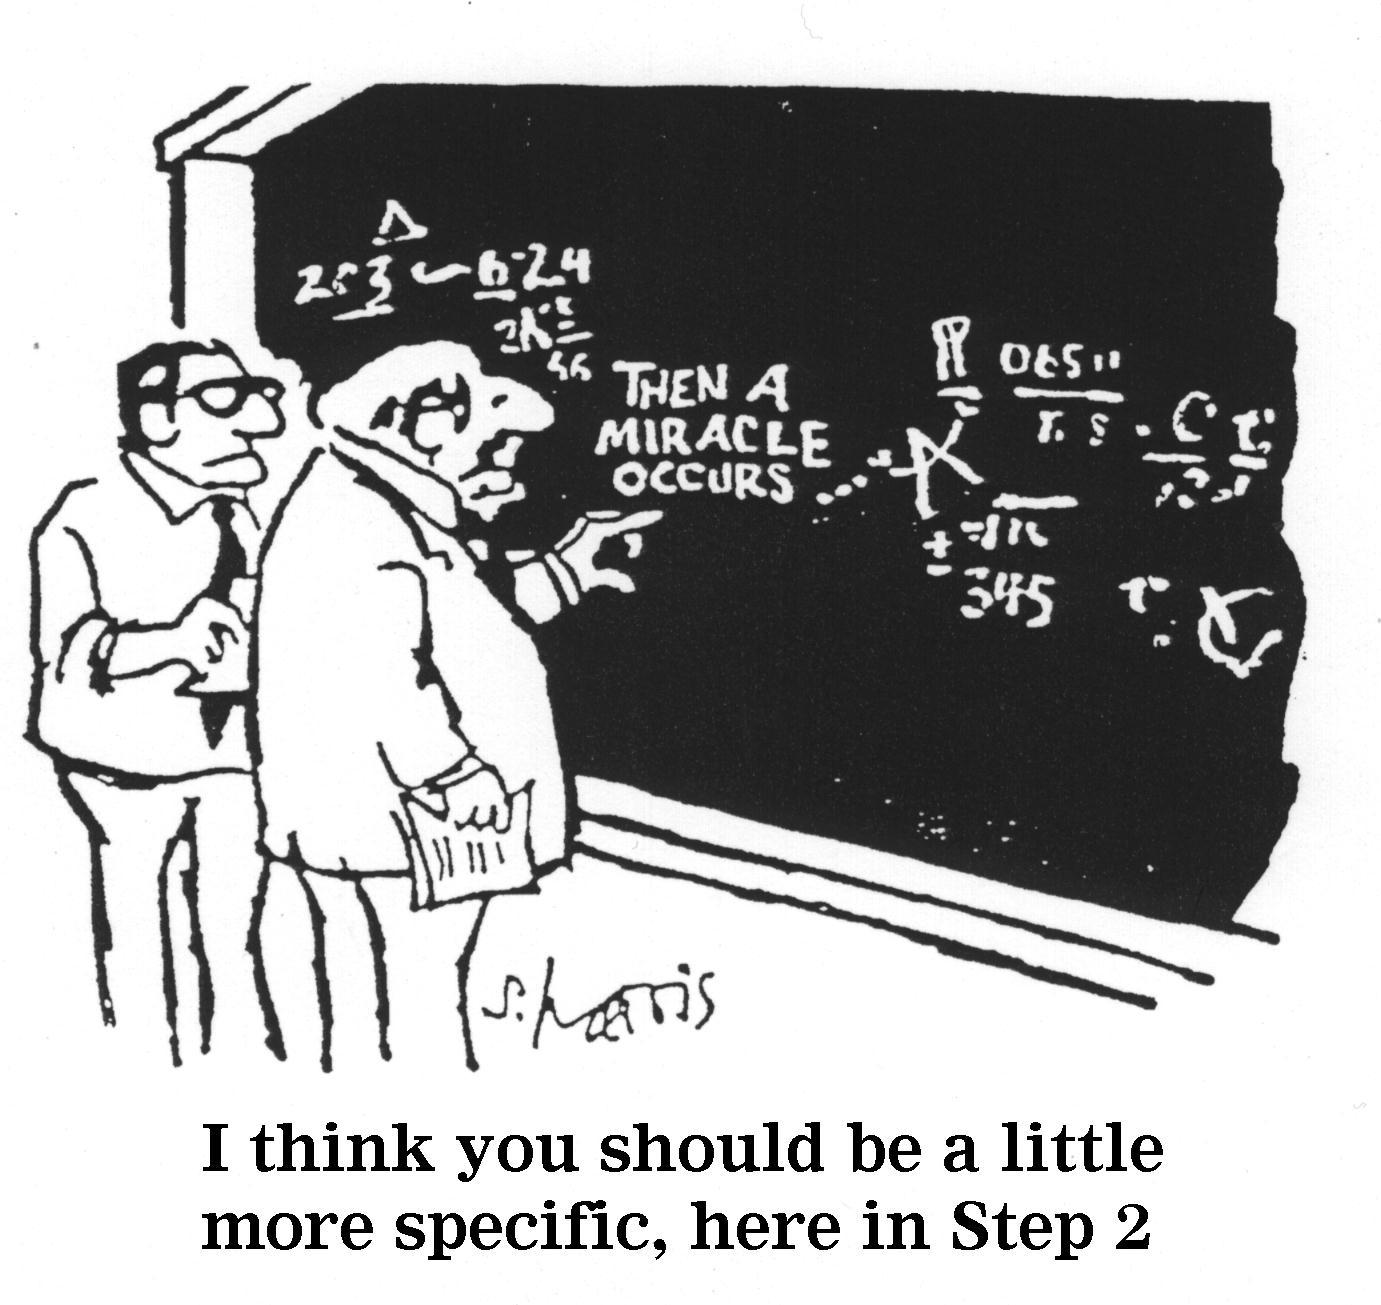
\includegraphics[width=0.4\textwidth]{images/miracle.jpeg}
\end{center}

But speculative execution inside your head is harder for perf than debugging.

So: we want to use tools \\ 
and do this in a methodical way.
\end{changemargin}

\end{frame}


%%%%%%%%%%%%%%%%%%%%%%%%%%%%%%%%%%%%%%%%%%%%%%%%%%%%%%%%%%%%%%%%%%%%%%%%%%%%%%%%
\begin{frame}
  \frametitle{Introduction to Profiling}



\begin{changemargin}{1.5cm}
    So far we've been looking at small problems.\\[1em]
    Must {\bf profile} to see what's slow in a
      large program.\\[1em]
    Two main outputs:
      \begin{itemize}
        \item flat;
        \item call-graph.
      \end{itemize}



    Two main data gathering methods:
      \begin{itemize}
        \item statistical;
        \item instrumentation.
      \end{itemize}
   \end{changemargin}
\end{frame}
%%%%%%%%%%%%%%%%%%%%%%%%%%%%%%%%%%%%%%%%%%%%%%%%%%%%%%%%%%%%%%%%%%%%%%%%%%%%%%%%

%%%%%%%%%%%%%%%%%%%%%%%%%%%%%%%%%%%%%%%%%%%%%%%%%%%%%%%%%%%%%%%%%%%%%%%%%%%%%%%%
\begin{frame}
  \frametitle{Profiler Outputs}


\begin{changemargin}{.5cm}
  
  {\bf Flat Profiler:}

  \begin{itemize}
    \item Only computes average time in a particular function.
    \item Does not include other (useful) information (callees).
  \end{itemize}

~\\[1em]

  {\bf Call-graph Profiler:}

  \begin{itemize}
    \item Computes call times.
    \item Reports frequency of function calls.
    \item Gives a call graph: who called what function?
  \end{itemize}
  \end{changemargin}
\end{frame}
%%%%%%%%%%%%%%%%%%%%%%%%%%%%%%%%%%%%%%%%%%%%%%%%%%%%%%%%%%%%%%%%%%%%%%%%%%%%%%%%

%%%%%%%%%%%%%%%%%%%%%%%%%%%%%%%%%%%%%%%%%%%%%%%%%%%%%%%%%%%%%%%%%%%%%%%%%%%%%%%%
\begin{frame}
  \frametitle{Data Gathering Methods}


\begin{changemargin}{1.5cm}
  {\bf Statistical:}

  Mostly, take samples of the system state, that is:
  \begin{itemize}
    \item every 100ms, check the system state.
    \item will cause some slowdown, but not much.
  \end{itemize}
~\\[1em]

  {\bf Instrumentation:}\\
  Add instructions at specified program points:
  \begin{itemize}
    \item can do this at compile time or run time (expensive);
    \item can instrument either manually or automatically;
    \item like conditional breakpoints.
  \end{itemize}
  \end{changemargin}
\end{frame}
%%%%%%%%%%%%%%%%%%%%%%%%%%%%%%%%%%%%%%%%%%%%%%%%%%%%%%%%%%%%%%%%%%%%%%%%%%%%%%%%

%%%%%%%%%%%%%%%%%%%%%%%%%%%%%%%%%%%%%%%%%%%%%%%%%%%%%%%%%%%%%%%%%%%%%%%%%%%%%%%%
\begin{frame}
  \frametitle{Guide to Profiling}

  

\begin{changemargin}{1cm}
  When writing large software projects:\\[1em]

     $\bullet$ First, write clear and concise code. \\
      \qquad Don't do premature optimizations---\\
      \qquad focus on correctness.\\
     $\bullet$ Profile to get a baseline of your performance:\\[0em]
      \begin{itemize}
        \item allows you to easily track any performance changes;
        \item allows you to re-design your program before it's too late.
      \end{itemize}
  Focus your optimization efforts on the code that matters.
  \end{changemargin}
\end{frame}
%%%%%%%%%%%%%%%%%%%%%%%%%%%%%%%%%%%%%%%%%%%%%%%%%%%%%%%%%%%%%%%%%%%%%%%%%%%%%%%%

%%%%%%%%%%%%%%%%%%%%%%%%%%%%%%%%%%%%%%%%%%%%%%%%%%%%%%%%%%%%%%%%%%%%%%%%%%%%%%%%
\begin{frame}
  \frametitle{Things to Look For}


\begin{changemargin}{1.5cm}
  
    Good signs:\\[0em]

    \begin{itemize}
      \item Time is spent in the right part of the system.
      \item Most time should not be spent handling errors;\\
 in non-critical code; or in exceptional cases.
      \item Time is not unnecessarily spent in OS.
    \end{itemize}
    \end{changemargin}
    
    \begin{center}
	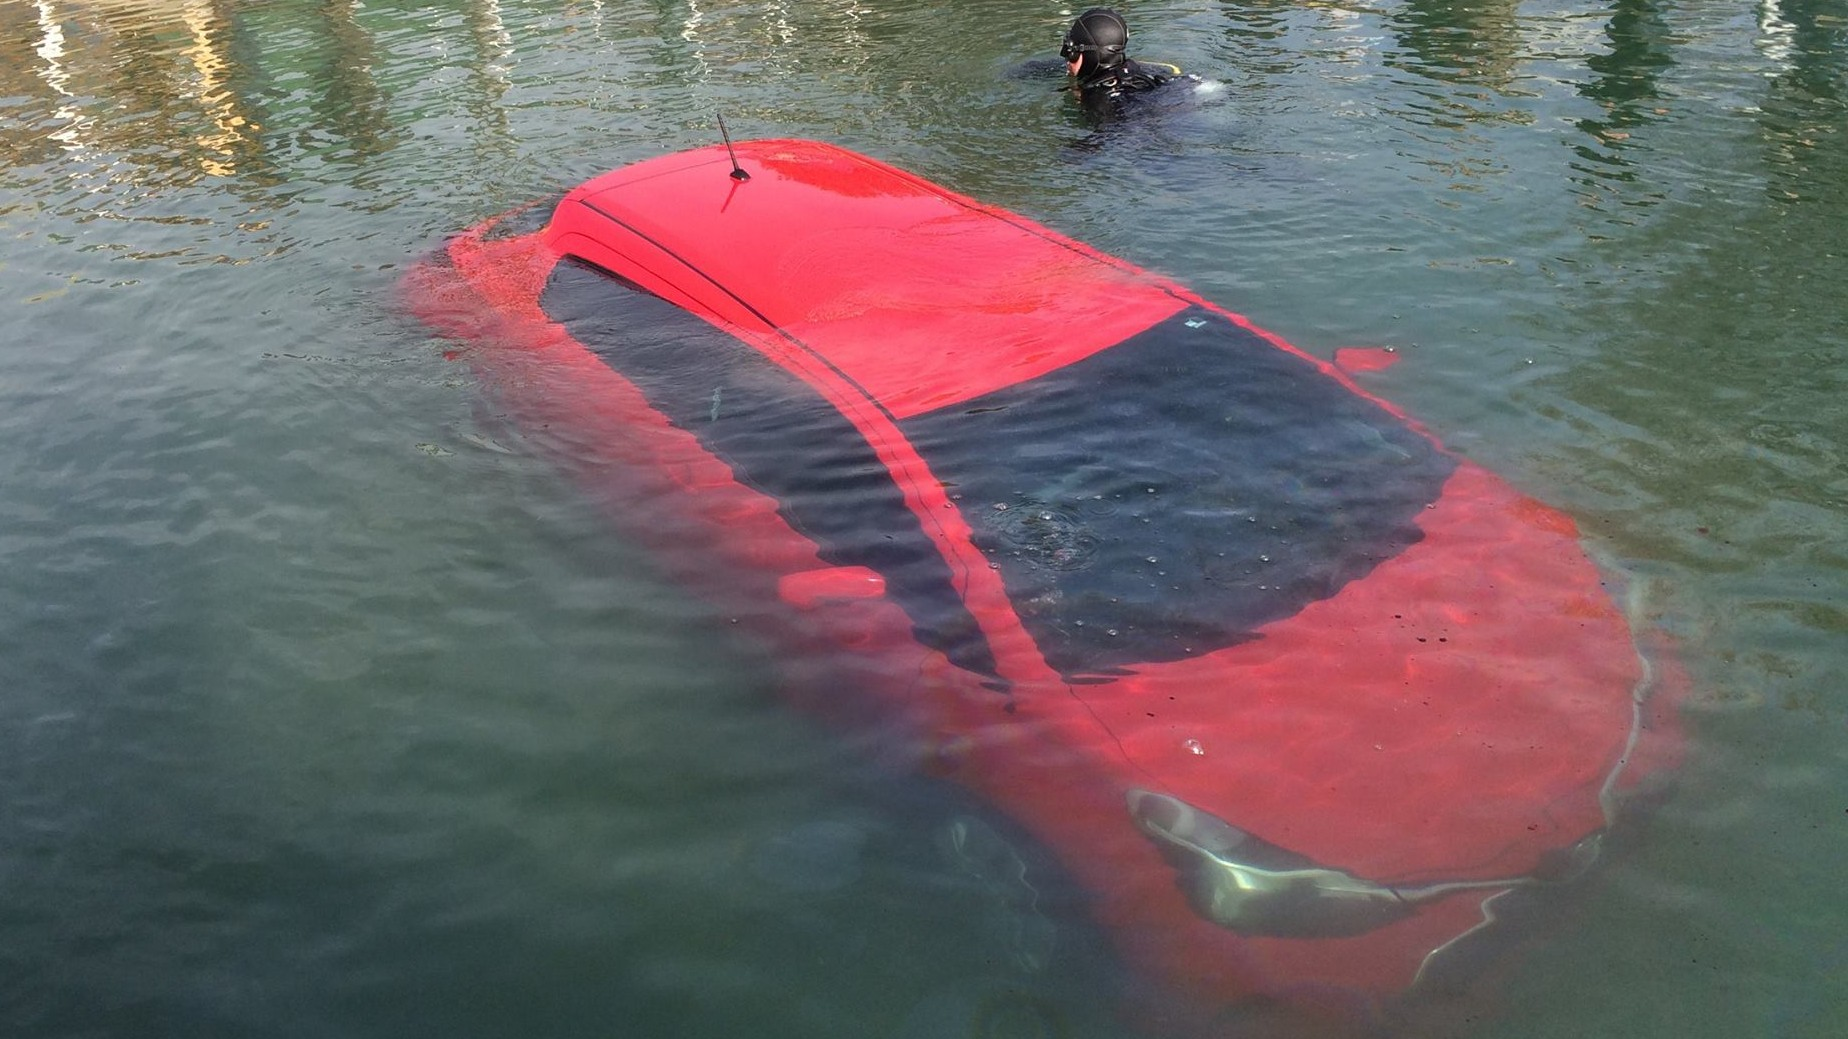
\includegraphics[width=0.5\textwidth]{images/tobermory.jpg}\\
	\hfill Kitchener driver follows GPS directions right into Lake Huron...
 	\end{center}
    
\end{frame}
%%%%%%%%%%%%%%%%%%%%%%%%%%%%%%%%%%%%%%%%%%%%%%%%%%%%%%%%%%%%%%%%%%%%%%%%%%%%%%%%


\begin{frame}
\frametitle{Development vs Prod}

You can always profile your systems in development, but that might not
help with complexities in production. 

The constraints on profiling 
production systems are that the profiling must not affect the system's
performance or reliability.


\end{frame}


\begin{frame}
\frametitle{Per-Process}

 We'll first talk about {\tt perf}, the profiler 
recommended for use with Rust. This is Linux-specific, though.

The \texttt{perf} tool is an interface to the Linux kernel's built-in
sample-based profiling using CPU counters. 

\end{frame}


\begin{frame}[fragile]
\frametitle{Previous Offering Profiling}

\begin{lstlisting}[basicstyle=\scriptsize]
[plam@lynch nm-morph]$ perf stat ./test_harness

 Performance counter stats for './test_harness':

       6562.501429 task-clock                #    0.997 CPUs utilized          
               666 context-switches          #    0.101 K/sec                  
                 0 cpu-migrations            #    0.000 K/sec                  
             3,791 page-faults               #    0.578 K/sec                  
    24,874,267,078 cycles                    #    3.790 GHz                     [83.32%]
    12,565,457,337 stalled-cycles-frontend   #   50.52% frontend cycles idle    [83.31%]
     5,874,853,028 stalled-cycles-backend    #   23.62% backend  cycles idle    [66.63%]
    33,787,408,650 instructions              #    1.36  insns per cycle        
                                             #    0.37  stalled cycles per insn [83.32%]
     5,271,501,213 branches                  #  803.276 M/sec                   [83.38%]
       155,568,356 branch-misses             #    2.95% of all branches         [83.36%]

       6.580225847 seconds time elapsed
\end{lstlisting} %$

\end{frame}

\begin{frame}[fragile]
\frametitle{Do it with Rust}

The first thing to do is to compile with debugging info, go to your \texttt{Cargo.toml} file and add:
\begin{verbatim}
[profile.release]
debug = true
\end{verbatim}

This means that \verb+cargo build --release+ will now compile the version with debug info.

\end{frame}

\begin{frame}
\frametitle{I've got a Cunning Plan}

Run the program using \texttt{perf record}, which will sample the execution of the program to produce a data set.


Then there are three ways we can look at the code: \texttt{perf report}, \texttt{perf annotate}, and a flamegraph.

\end{frame}


\begin{frame}
\frametitle{CLion}

During development of some of the code exercises, I used the CLion built-in profiler for this purpose. 

It generates a flamegraph for you too, and I'll show that for how to create the flamegraph as well.


\end{frame}

\part{Profiler Guided Optimization}
\begin{frame}
\partpage
\end{frame}

\begin{frame}[fragile]
\frametitle{Profiler Guided Optimization}


Using static analysis, \\
the compiler makes its best predictions about runtime behaviour.

Example: branch prediction. 

\begin{lstlisting}[language=Rust]
fn which_branch(a: i32, b: i32) {
    if a < b {
        println!("Case one.");
    } else {
        println!("Case two.");
    }
}
\end{lstlisting}

\end{frame}

\begin{frame}[fragile]
\frametitle{A Virtual Call to Devirtualize}

\begin{multicols}{2}
\begin{lstlisting}[language=Rust]
trait Polite {
    fn greet(&self) -> String;
}

struct Kenobi {
    /* Stuff */
}
impl Polite for Kenobi {
    fn greet(&self) -> String {
        return String::from("Hello there!");
    }
}
\end{lstlisting}
\columnbreak
\begin{lstlisting}[language=Rust]
struct Grievous {
    /* Things */
}
impl Polite for Grievous {
    fn greet(&self) -> String {
        return String::from("General Kenobi.");
    }
}

fn devirtualization(thing: &Polite) {
    println!("{}", thing.greet());
}

\end{lstlisting}
\end{multicols}

\end{frame}


\begin{frame}[fragile]
\frametitle{Match}

\begin{lstlisting}[language=Rust]
fn match_thing(x: i32) -> i32 {
    match x {
        0..10 => 1,
        11..100 => 2,
        _ => 0
    }
}
\end{lstlisting}

Same thing with \texttt{x}: what is its typical value? If we know that, it is our prediction. 

Actually, in a match block with many options, could we rank them in descending order of likelihood?

\end{frame}


\begin{frame}
\frametitle{Adapting to an Uncertain World}


How can we know where we go?
\begin{itemize}
\item could provide hints\ldots
\end{itemize}

Java HotSpot virtual machine: updates predictions on the fly. 

So, just guess.\\
If wrong, the Just-in-Time compiler adjusts \& recompiles.

The compiler runs and it does its job and that's it; the program is never updated with newer predictions if more data becomes known.


\end{frame}



\begin{frame}
\frametitle{Profiling Mitigates Uncertainty}



Rust: usually no adaptive runtime system.

POGO:
\begin{itemize}
\item observe actual runs;
\item predict the future.
\end{itemize}

So, we need multi-step compilation:
\begin{itemize}
\item compile with profiling;
\item run to collect data;
\item recompile with profiling data to optimize.
\end{itemize}



\end{frame}



\begin{frame}
\frametitle{Step One: Measure}



First, generate an executable with instrumentation. 

The compiler inserts a bunch of probes into the generated code to record data. 
\begin{itemize}
\item Function entry probes;
\item Edge probes;
\item Value probes.
\end{itemize}

Result: instrumented executable plus empty database file (for profiling data).


\end{frame}



\begin{frame}
\frametitle{Step Two: Training Day}

\begin{center}
	
\includegraphics[width=0.6\textwidth]{images/training-day.jpg}
\end{center}

\end{frame}


\begin{frame}
\frametitle{Step Two: Training Day}



Second, run the instrumented executable.

Real-world scenarios are best.

Ideally, spend training time on perf-critical sections. 

Use as many runs as you can stand.

\end{frame}



\begin{frame}
\frametitle{Step Two: Training Day}



Don't exercise every part of the program (not SE 465/ECE 453 here!)

That would be counterproductive.

Usage data must match real world scenarios,\\
... or the compiler gets misinformed about what's important. 

Or you might end up teaching it that almost nothing
is important\ldots (``everything's on the exam!'')


\end{frame}



\begin{frame}
\frametitle{Step Three: Recompile}



Finally, compile the program again.

Inputs: source plus training data.

Outputs: (you hope) a better output executable than from static analysis alone.


\end{frame}



\begin{frame}
\frametitle{Summary Graphic}

\begin{center}
	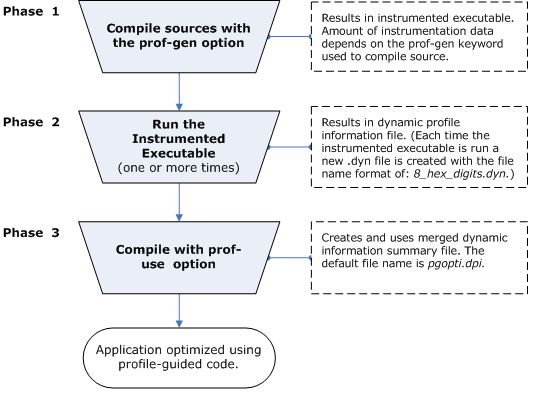
\includegraphics[width=0.75\textwidth]{images/pogo-workflow.jpg}
\end{center}

\end{frame}



\begin{frame}
\frametitle{Save Some Steps}



Not necessary to do all three steps for every build. 

Re-use training data while it's still valid.

Recommended dev workflow:
\begin{itemize}
\item dev A performs these steps, checks the training data into source control
\item whole team can use profiling information for their compiles.
\end{itemize}


\end{frame}



\begin{frame}
\frametitle{Not fixing all the problems in the world}



What does it mean for it to be better? 

The algorithms will aim for speed in areas that are ``hot''. 

The algorithms will aim for minimal code size in areas that are ``cold'' .

Less than 5\% of methods compiled for speed.

\end{frame}



\begin{frame}
\frametitle{Combining Training Runs}



Can combine multiple training runs and manually give suggestions about important scenarios.

The more a scenario runs in the training data, \\
the more important it will be, from POGO's point of view.

Can merge multiple runs with user-assigned weightings.


\end{frame}


\begin{frame}[fragile]
\frametitle{Full Test Scenario}

{\scriptsize
\begin{verbatim}
# STEP 1: Compile the binary with instrumentation
rustc -Cprofile-generate=/tmp/pgo-data -O ./main.rs

# STEP 2: Run the binary a few times, maybe with common sets of args.
#         Each run will create or update `.profraw` files in /tmp/pgo-data
./main mydata1.csv
./main mydata2.csv
./main mydata3.csv

# STEP 3: Merge and post-process all the `.profraw` files in /tmp/pgo-data
llvm-profdata merge -o ./merged.profdata /tmp/pgo-data

# STEP 4: Use the merged `.profdata` file during optimization. All `rustc`
#         flags have to be the same.
rustc -Cprofile-use=./merged.profdata -O ./main.rs
\end{verbatim}
}

\end{frame}



\begin{frame}
\frametitle{Behind the Scenes}



In the optimize phase, compiler uses the training data for:

\begin{enumerate}
\item Full and partial inlining
\item Function layout
\item Speed and size decision
\item Basic block layout 
\item Code separation
\item Virtual call speculation
\item Switch expansion
\item Data separation
\item Loop unrolling
\end{enumerate}

\end{frame}



\begin{frame}
\frametitle{Muh Gainz}



Most performance gains from inlining.

Decisions based on the call graph path profiling. 

But: behaviour of function \texttt{foo} may be very different when called from \texttt{B} than when called from \texttt{D}. 


\begin{center}
	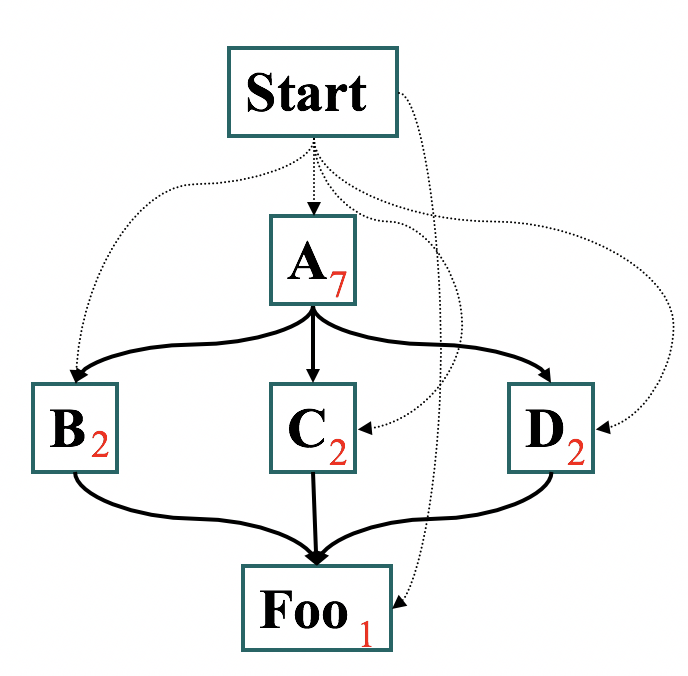
\includegraphics[width=0.4\textwidth]{images/callpaths.png}
\end{center}

\end{frame}



\begin{frame}
\frametitle{Another Call Graph}


Example 2 of relationships between functions.\\
Numbers on edges represent the number of invocations:

\begin{center}
	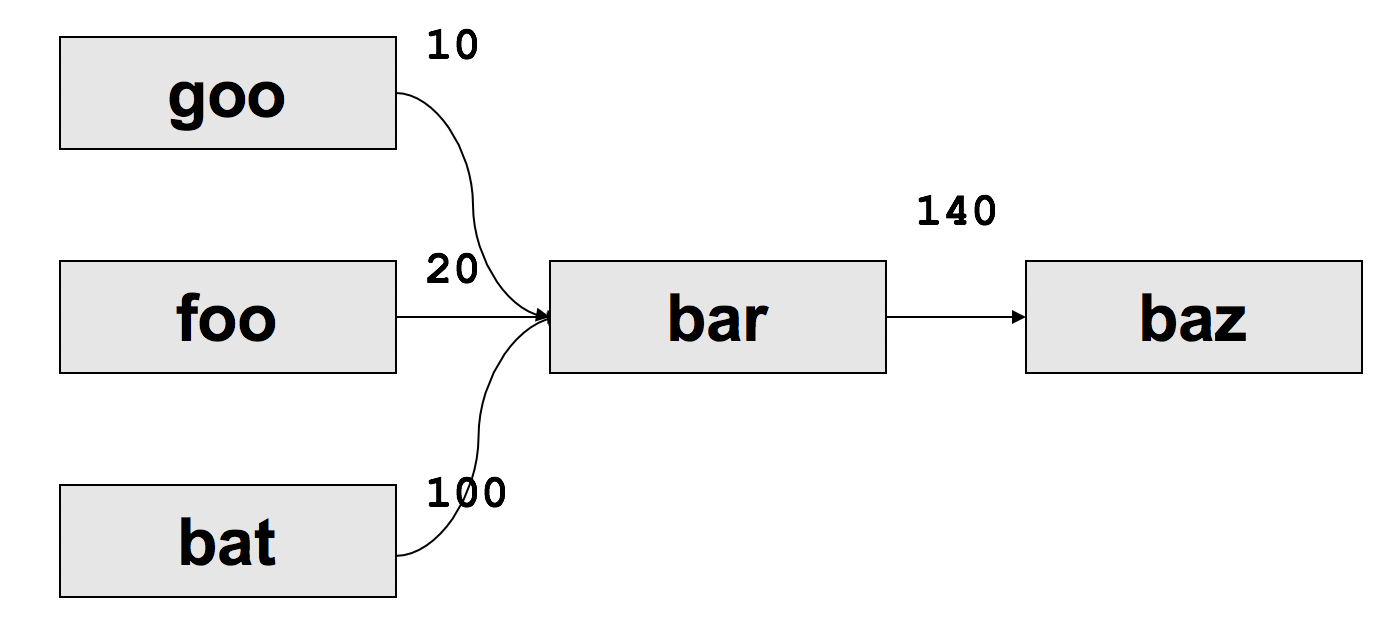
\includegraphics[width=\textwidth]{images/callpaths2.png}
\end{center}

\end{frame}



\begin{frame}
\frametitle{The POGO View of the World}

When considering what to do here, POGO takes the view like this:

\begin{center}
	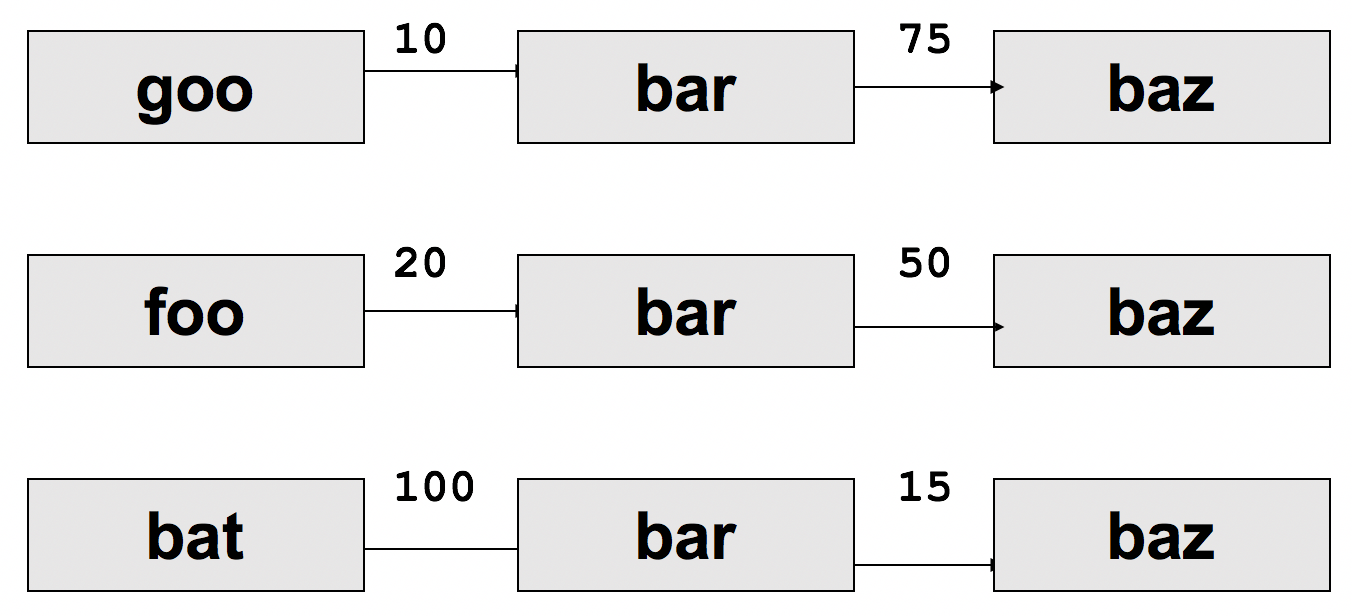
\includegraphics[width=\textwidth]{images/callpaths3.png}
\end{center}

\end{frame}



\begin{frame}
\frametitle{The POGO View of the World}

\begin{center}
	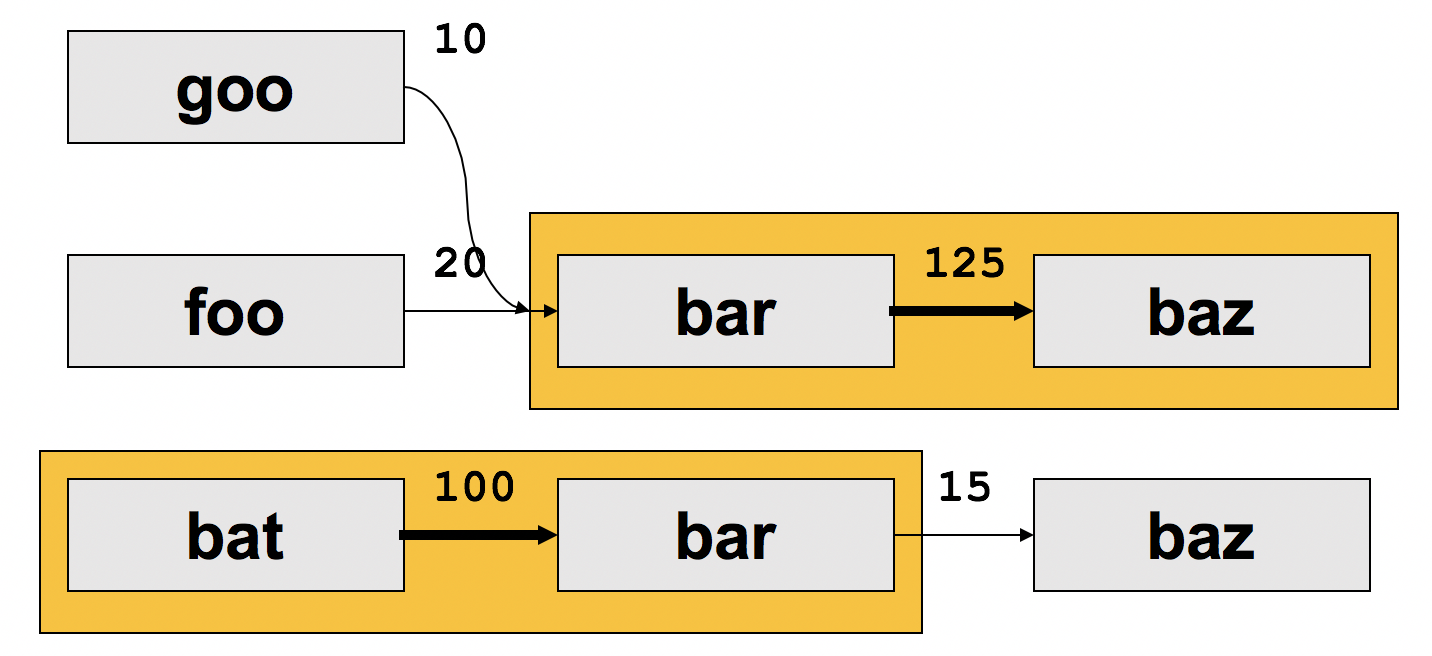
\includegraphics[width=\textwidth]{images/callpaths4.png}
\end{center}

\end{frame}




\begin{frame}
\frametitle{Page Locality}



Call graph profiling data also good for packing blocks.

Put most common cases nearby.\\
Put successors after their predecessors.

Packing related code = fewer page faults (cache misses).

Calling a function in same page as caller =  ``page locality''.


\end{frame}



\begin{frame}
\frametitle{Block Layout}

\begin{center}
	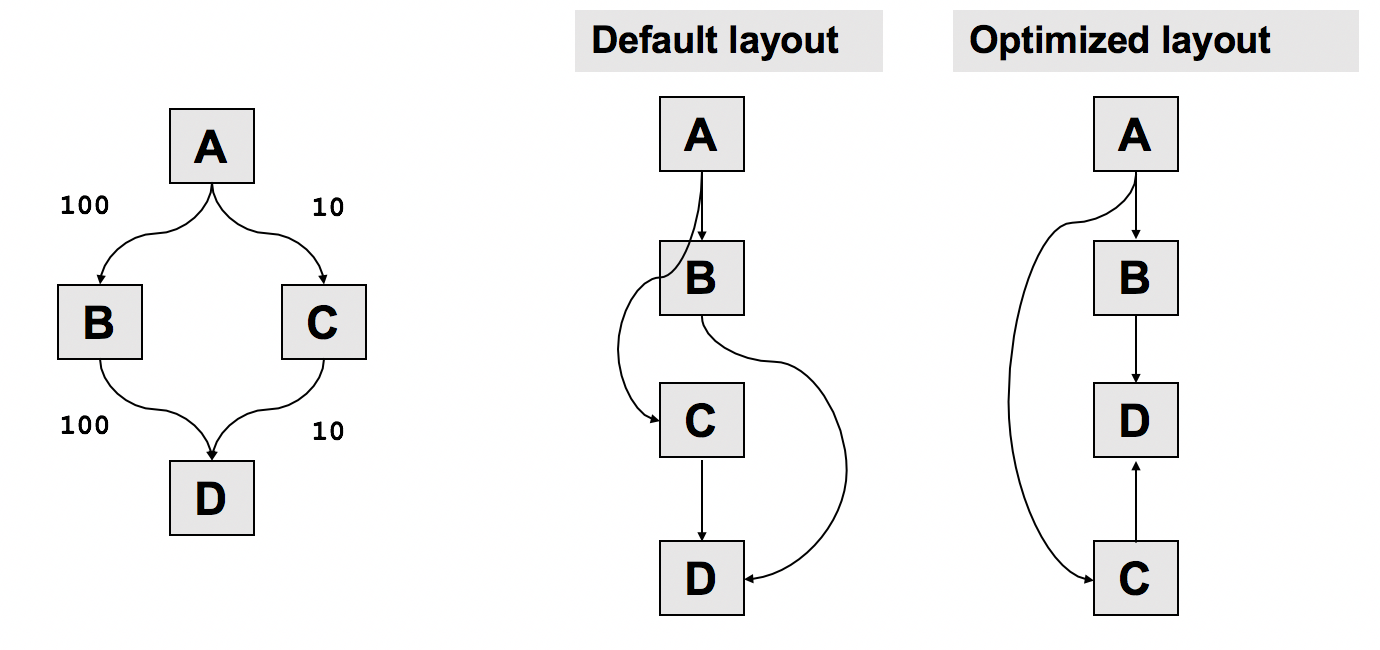
\includegraphics[width=\textwidth]{images/blocklayout.png}
\end{center}

\end{frame}



\begin{frame}
\frametitle{Dead Code?}



According to the author, ``dead'' code goes in its own special block. 

Probably not truly dead code (compile-time unreachable).

Instead: code that never gets invoked in training.


\end{frame}



\begin{frame}
\frametitle{Benchmark Results}
 
OK, how well does POGO work?

The application under test is a standard benchmark suite (Spec2K):


\begin{center}
\begin{tabular}{l|l|l|l|l|l}
	\textbf{Spec2k:} & \textbf{sjeng} & \textbf{gobmk} & \textbf{perl} & \textbf{povray} & \textbf{gcc}\\ \hline
	\textbf{App Size:} &  {Small} & {Medium} & {Medium} & {Medium} & {Large} \\ \hline
	\textbf{Inlined Edge Count} & 50\% & 53\% & 25\% & 79\% & 65\% \\ \hline
	\textbf{Page Locality} & 97\% & 75\% & 85\% & 98\% & 80\% \\ \hline
	\textbf{Speed Gain} & 8.5\% & 6.6\% & 14.9\% & 36.9\% & 7.9\% \\ 
\end{tabular}
\end{center}

 
We can speculate about how well synthetic benchmarks results translate to real-world application performance\ldots


\end{frame}




\end{document}

